% !TeX root = ../SDonchezThesis.tex

\chapter{Memory and Peripheral Isolation for Tenant Data Integrity}\label{ch:dmaProtection}
Although the EDF Algorithm outlined in the preceding chapter enables the efficient decryption of tenant bitstreams with shared decryption engines, the encrypted transmission of the bitstream is itself useless if any co-tenant on the PFPGA is granted access to the decrypted bitstream as stored in RAM. To this end, it is imperative that memory isolation functionality be utilized throughout the PFPGA to limit each tenant's partition to only the portions of the memory space that are allocated to said tenant. Similarly, care should be taken to re-allocate access permissions to the decryption engines as they change tasks, such that the end user can be guaranteed that access only persists through the decryption partition for as long as is necessary. Finally, the static partition, containing the CSP's supervisory functionality and resources, should be, to the maximum extent practical, isolated from the tenant data (although the presence of the HPS interface and the DDR controller interface in this region necessitate some amount of unrestricted access).

To this end, the architecture presented in Chapter \ref{ch:systemArchitecture} incorporates the use of Xilinx Memory and Peripheral Protection Units for Programmable Logic Isolation (XMPU-PL), as proposed in \cite{noauthor_memory_2021}. By combining these cores with individual AXI interconnect switches for each partition, and configuring the Region parameters of each core according to the partition it is located in, total isolation can be achieved provided that the static bitstream is from a known and trusted source (as has been outlined elsewhere in this work).

The remainder of this chapter outlines the implementation of this mechanism in the programmable logic. It begins with a discussion of the relevant background material and other academic work in the area. It then outlines in detail the proposed design, and concludes with a discussion of its implementation and the results of testing.

\section{Background}\label{sec:DMABackground}

The idea of a need for some form of system isolation in an embedded system is not a new one. ARM-based systems have implemented a technology called ``TrustZone'' for several generations, which establishes the concept of a ``Secure World'' and a ``Non-Secure World'' within the processing system. In a TrustZone enabled system, non-secure components are prohibited from accessing secured resources, while the ability of a secure component to access a non-secure resource is configurable. This enables a basic isolation scheme, wherein a secure supervisor can oversee the execution of non-secure applications, without concerns that malicious non-secure applications could compromise the resources of the secure supervisor. Xilinx and many other FPGA vendors have also devised a system whereby TrustZone (or Intel's SGX, or any other equivalent system) can be extended into the programmable logic, with certain devices assigned as secure while others are not. 

Xilinx has furnished several documents discussing the isolation of memory and peripherals in an MPSoC architecture. Their flagship line of MPSoC devices, the Zynq UltraScale+ series, implements a number of Xilinx Memory Protection Units (XMPUs) in conjunction with Xilinx Peripheral Protection Units (XPPUs) to enable the strict isolation of various portions of the system if desired. Figure \ref{fig:XMPPUs} indicates these units within the larger MPSoC architecture, with the XMPU and XPPU cores highlighted in red. \cite{mcneil_isolation_2021} provides a detailed explanation of the use of these units in an MPSoC to afford isolation of domains, as well as a comprehensive discussion of their implementation and limitations.

\begin{figure}[h]
    \centering
    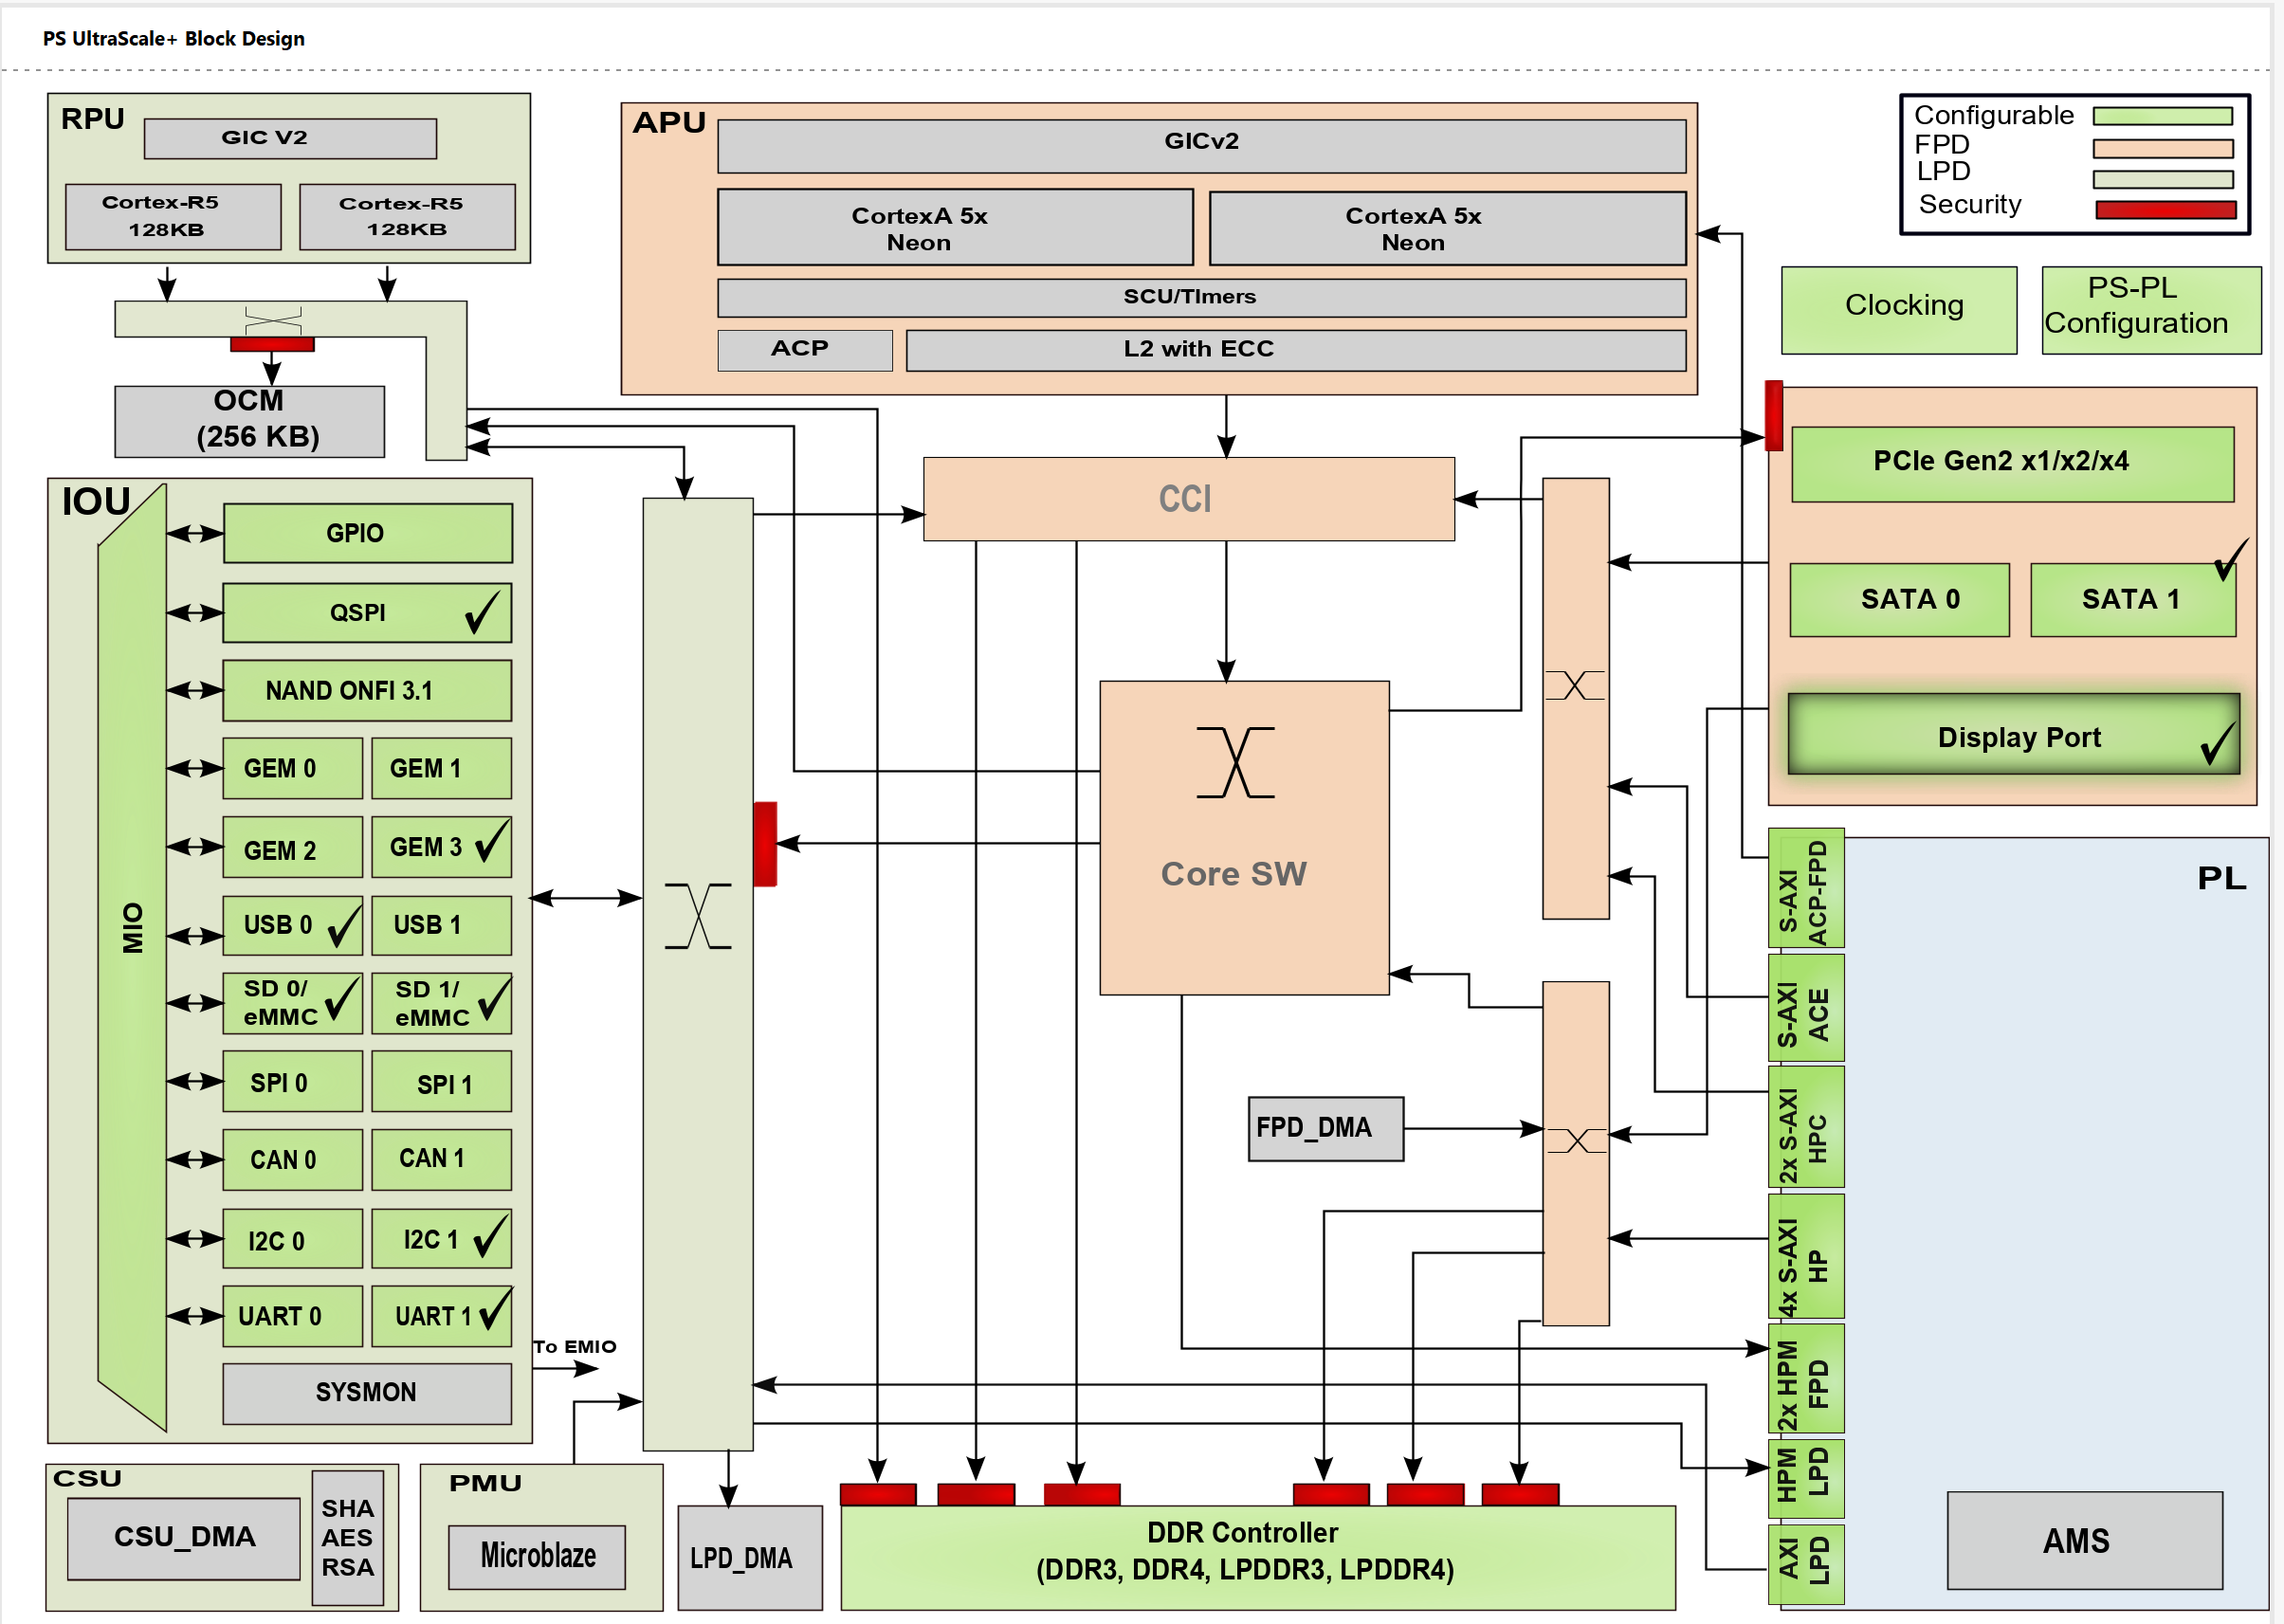
\includegraphics[width=0.8\textwidth]{USP_XMPUs}
    \caption [XMPU and XPPUs in a Zynq UltraScale+]{Xilinx Memory Protection Units (XMPUs) and Xilinx Peripheral Protection Units (XPPUs) within the Zynq UltraScale+ MPSoC architecture}
    \label{fig:XMPPUs}
\end{figure}

Unfortunately, this binary configuration is unsuitable for a multi-tenant configuration. Although there is a need for the supervisory mechanism (furnished by the CSP or the FPGA Vendor) to remain isolated from tenant components, there is also a need for isolation between different tenant components, a flexibility which is not afforded by TrustZone or its competitors. Instead, some form of more granular memory and peripheral isolation is required.

Many of the academic works that have been published on the topic of multi-tenant FPGA-based systems (such as those discussed in Section \ref{sec:LitImpl} have, at the least, acknowledged the need for memory isolation as a means of ensuring tenant data confidentiality and integrity. Unfortunately, many of these discussions are abstract in nature, and lack concrete implementation. For example, \cite{bag_cryptographically_2020} places the responsibility for memory isolation on the OpenStack architecture they base their design on, without a robust consideration of the application of this isolation to the programmable logic. Meanwhile, \cite{chen_enabling_2014} outlines a detailed plan for memory isolation, but does so by utilizing a processor based virtual environment for each partition, imposing appreciable system overhead while not guaranteeing isolation from malicious cotenants on the programmable logic.

As is evident from Figure \ref{fig:XMPPUs}, the XPPU and XMPU cores are used to enable the isolation of various key portions of the system, including the processors, IO, and various memory devices. However, it is important to note the absence of any isolation functionality within the programmable logic itself, which, tied with the practice of ``memory mapping'' various PL based logic devices, leaves an avenue for malicious co-tenants within the programmable logic to gain access to other tenants' IP. In \cite{noauthor_memory_2021}, Xilinx proposes the aforementioned XMPU-PL IP, which enables the previously absent isolation of memory-mapped PL devices at a granular level. A block diagram of this component is shown in Figure \ref{fig:XMPU_PL_BD}. Unfortunately, neither of these Xilinx references address the specific task of this effort, facilitating multiple mutually untrustworthy tenant on a single system. Rather, they propose a strict linear trust model that does not entertain the concept of multiple entities requiring equal but separate permissions.

\begin{figure}[h]
    \centering
    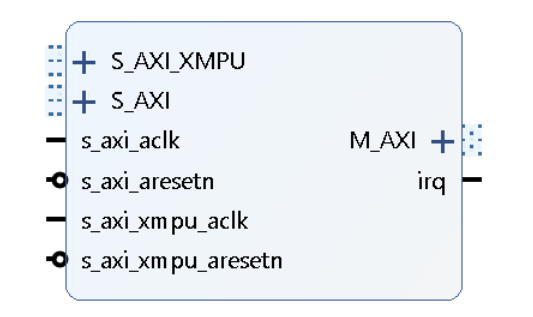
\includegraphics[width=0.5\textwidth]{XMPU_PL_Symbol}
    \caption [XMPU-PL IP Core]{Vivado Representation of the XMPU-PL IP \cite{noauthor_memory_2021}}
    \label{fig:XMPU_PL_Sym}
\end{figure}


%This work utilizes these XMPU-PL units to dynamically confine the decryption engines' memory access to whatever tenant partition they are currently processing encrypted bitstream data for (as determined by the scheduling engine outlined in Chapter \ref{ch:edfScheduling}). It also utilizes the XMPU-PLs to serve as a ``gate'' for all memory requests for each partition, thereby preventing a malicious actor from attempting to access other tenants' devices or memory space. By utilizing these XMPU-PL cores in an attestable bitstream (such as one provided by an FPGA vendor or trusted third party), the tenant can be assured of PL confidentiality and integrity.

The remainder of this chapter lays out a proposal to remedy this issue. First, it discusses the XMPU-PL core in detail, drawing heavily from reference designs presented in \cite{noauthor_memory_2021} and accompanying first-hand experimental results. Then, using a Trust-Zone based hierarchical separation between static components (such as the decryption engines), which form a portion of the bitstream provided from the trusted third party (FPGA vendor or independent trusted party), and tenant components withing their partition, the proposed design is able to ensure the integrity of the supervisory functions from a malicious tenant. Similarly, implementing XMPU-PL instances as a gateway for data flow into each tenant partition enables the partition to be strictly confined to its assigned memory space, and, additionally, allows the tenant to chose which peripherals to grant access to its partition. This last step is crucial to unlocking the full potential of FPGAs in a heterogenous environment, as they necessarily require interface with the other parts of the system in able to provide maximum usability.

\section{The XMPU-PL IP Core}

\begin{figure}[h]
    \centering
    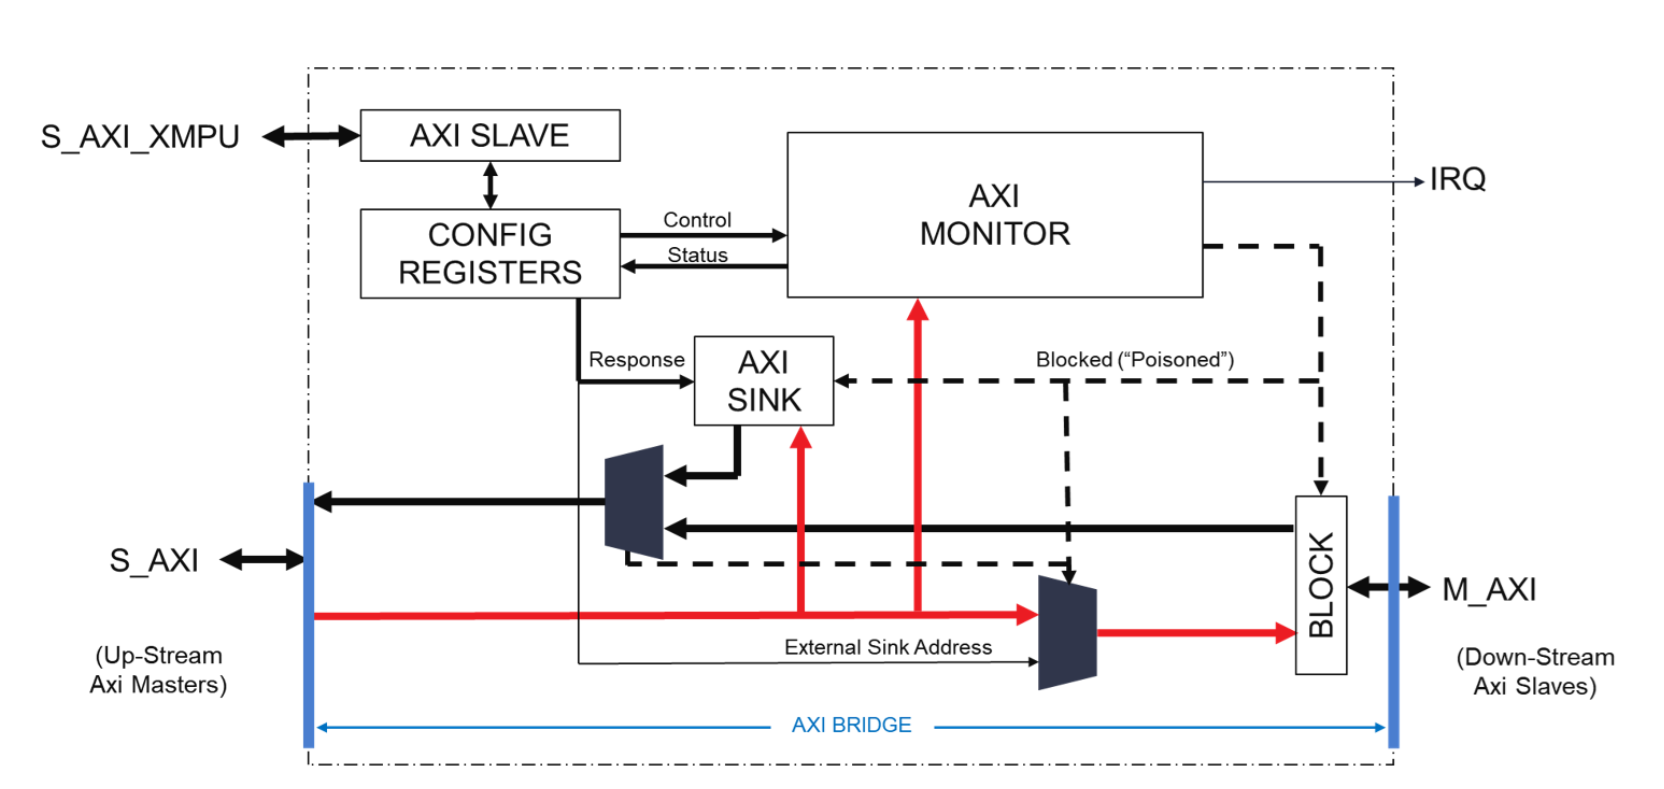
\includegraphics[width=0.8\textwidth]{XMPU_PLBlockDiagram}
    \caption [XMPU-PL Block Diagram]{Block diagram of the XMPU-PL IP \cite{noauthor_memory_2021}}
    \label{fig:XMPU_PL_BD}
\end{figure}

The XMPU-PL IP Core allows for the selective transit of AXI transactions from an Up-Stream AXI Master to Down-Stream AXI Slaves (as well as any responses flowing the other direction, i.e. data in response to a read request). The core extends the binary protection afforded by the TrustZone architecture by allowing address-restricted access to the AXI Slave Device. To achieve this, the core allows for the customization of up to 16 distinct regions of memory space, via the customization interface depicted in Figure \ref{fig:XMPU_region_config}. When configured, the XMPU-PL allows transactions to flow that are targeted at the given region if and only if the originating AXI Master is explicitly enabled in the ``Region XX Masters'' register. This register allows for the selective access of any of 32 distinct AXI Masters, including the various PS processors and interfaces. 

\begin{figure}[h]
    \centering
    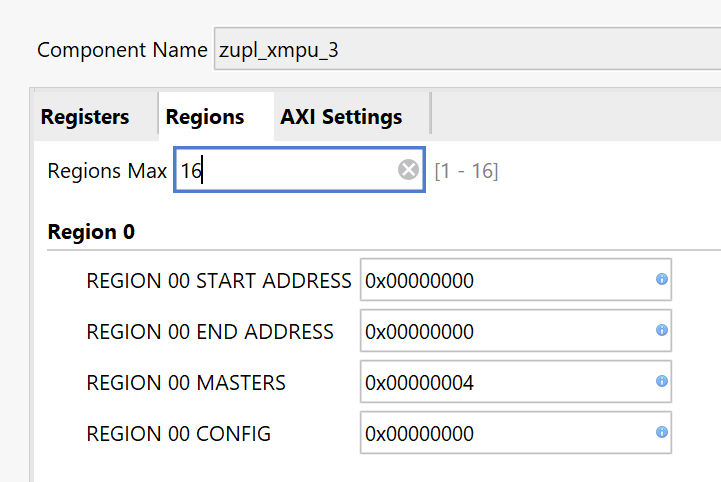
\includegraphics[width=0.5\textwidth]{XMPU_region_config}
    \caption[XMPU Region Configuration]{Configuration of the XMPU-PL IP}
    \label{fig:XMPU_region_config}
\end{figure}

In conjunction with address based filtering, each region can be configured with a TrustZone-based Secure or Non-Secure security level. By using this functionality, in conjunction with the ARM TrustZone based isolation of the trusted components from the untrusted, it is possible to completely restrict access to sensitive components, such as the decryption engines, to only those components that are explicitly enabled in the XMPU-PL. A full list of supported AXI Masters is presented in Appendix \ref{apx:axi-masters}.

Unfortunately, AXI Master-based verification only works against the specific AXI Masters pre-defined in the given register. This is due to an inherent design decision, whereby PL-based AXI Masters don't specify a Master ID in their transactions, making such differentiation impossible. Fortunately, the core can still be utilized as a combination of a TrustZone-based and memory region-based isolation mechanism in such an instance. This is done by modifying a pair of configuration parameters of the core, DefRdAllowed and DefWrAllowed, which control the behavior of the core when responding to requests that do not match any region defined in the region configuration registers. By setting these to their ``deny'' state, the core will deny all transactions that do not match any region defined in these registers, effectively preventing any access to memory regions that are not intended to be visible to the PL Master.

An additional feature afforded by the core is the ability to either statically or dynamically configure it. It is possible to provide design-time values to all of the registers utilized to control the core, and furthermore to lock those registers such that run-time modification is impossible. In this way, no additional setup overhead is required on the part of PS-based applications, and a malicious actor cannot compromise the integrity of the core by altering its isolation configuration. Alternatively, the registers can be exposed via a dedicated configuration AXI interface, enabling flexibility while also allowing only specific portions of the system to perform such updates.

Further register flags enable the implementer to customize the behavior of the core. For example, the response provided to an invalid request can be configured as one of several AXI status codes, ranging from an ``OK'' status to various error codes, some of which intentionally misrepresent the error as something other than a lack of permissions. Alternatively, such requests can be routed to a dedicated AXI Slave, such that custom responses can be provided. Additional registers allow for interrupt handling to allow for PS-PL communication.


\section{Isolation Lab Reference Designs}\label{sec:DMAIsolationLab}
The Xilinx document that proposes the XMPU-PL IP, \cite{noauthor_memory_2021}, includes a set of example ``Labs'', which enable the user to evaluate the functionality of the IP in an embedded environment. As part of this research effort, these designs, which were originally developed for the Xilinx ZCU102 development board, were modified for use on the AXU2CGB target specified in Section \ref{subsec:DMAEnvironmentHW}. This effort required a reconfiguration of the processor interface IP to account for the differing peripherals and memory controllers on the AXU2CGB target.

The tests provided by \cite{noauthor_memory_2021} provide tests of the XMPU-PL as part of a fully integrated isolated system. Such a system is configured via the processor interface IP's advanced configuration settings, as indicated in Figure \ref{fig:PS_int_isolation}. The reference design creates three partitions, one each for the Application Processor Unit (Cortex A processor cores), Real-Time Processor Unit (Cortex R processor cores), and the Power Management Unit (typically implemented as a MicroBlaze soft-processor, but not one that is user-generated). The design treats the PMU as the supervisory function of the system, with the RPU acting in a secured function while the APU performs untrusted functions.

\begin{figure}[h]
    \centering
    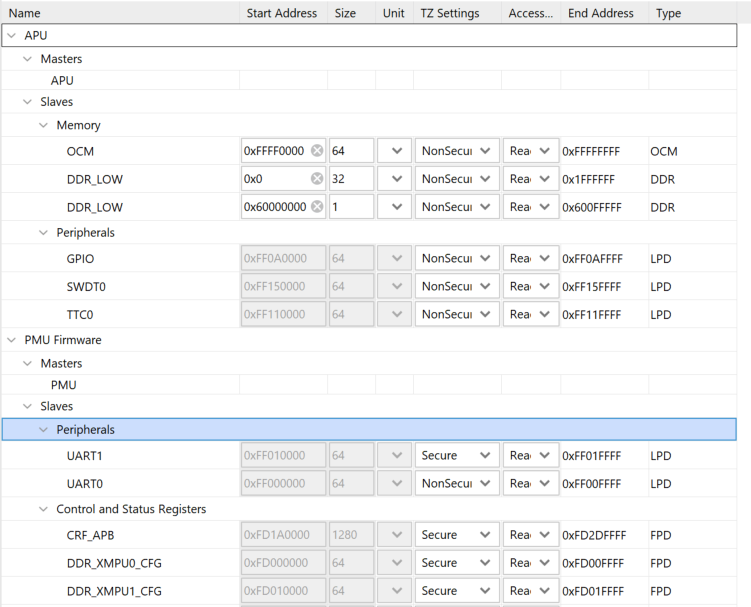
\includegraphics[width=0.8\textwidth]{PS_int_isolation}
    \caption{PS-PL Isolation Configuration}
    \label{fig:PS_int_isolation}
\end{figure}

\subsection{Lab Results}

In the example code accompanying \cite{noauthor_memory_2021}, Xilinx provides two sets of tests. Each utilizes the PMU as a supervisor, and both implement a First Stage Boot-loader (FSBL) on the RPU. However, one of the tests consists of attempts by the APU (which is non-secure), whereas the other exercises the XMPU (and other system components) from the RPU. As with the reference design itself, these tests required some modification in order to be run on the AXU2CGB target. Specifically, certain peripherals that are implemented on the larger ZCU102 target are not implemented on the AXU2CGB, and accordingly could not be integrated into the design (and accordingly, had to be removed from the test suite). 

Further modifications had to be made to account for the fact that the ZCU102 has a dual UART-over-USB interface that carries two serial channels, whereas the AXU2CGB only has one, which cannot be connected to the RPU subsystem due to design constraints. Fortunately, the target supports the transmission of a second UART over the JTAG interface, enabling monitoring of both the PMU in its supervisory role and the APU/RPU as they attempt to exercise it. Conversion of the JTAG interface on the AXU2CGB to a USB interface is accomplished using Alinx's ``USB Cable'', which, in keeping with the Xilinx device of the same name, is actually not a cable but instead its own complex PCB.

Using the two JTAG interfaces, one can view the results of attempts by the APU to compromise the secured PL components, as well as the PMU's response to these attempted violations. These results are captured in Figure \ref{fig:APU_Test_Suite}. As is shown in the figures, the APU is able to successfully access those memory regions (and memory-mapped devices) to which it is granted access (only a subset of which are shown for conciseness), but is unable to access the secure assets protected by the XMPU-PL core.

\begin{figure}[H]
    \centering
    \begin{subfigure}[b]{0.8\textwidth}
        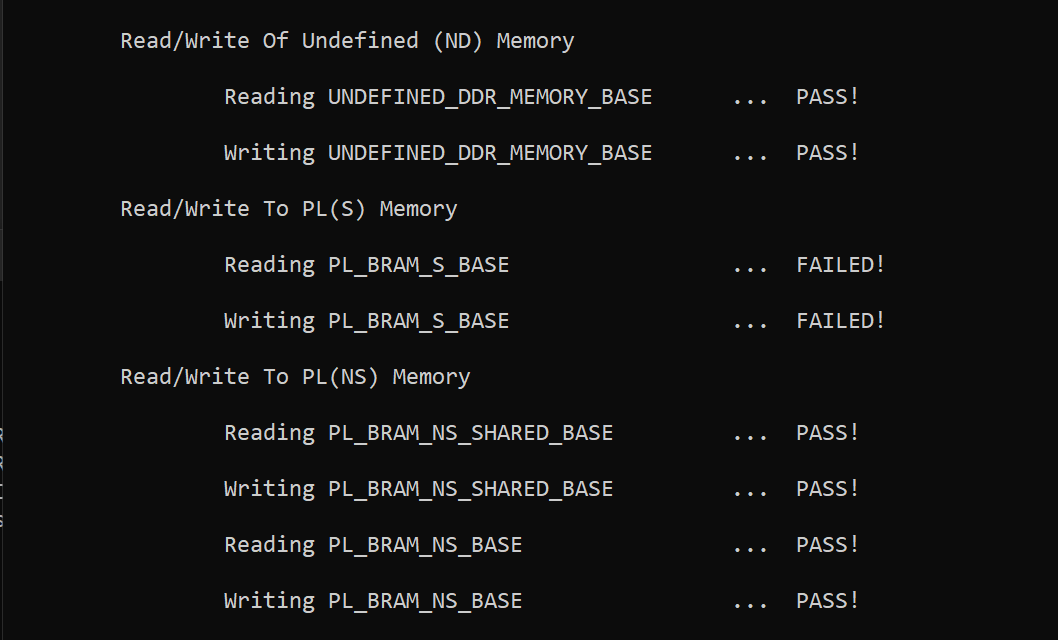
\includegraphics[width=\textwidth]{APU_FI/APU_PLReads}
        \caption{APU PL Read Attempt}
        \label{subfig:APU_PLRead}
    \end{subfigure}
\end{figure}
\begin{figure}[H]
    \ContinuedFloat
    \centering
    \begin{subfigure}[b]{0.8\textwidth}
        \includegraphics[width=\textwidth]{APU_FI/PMU}
        \caption{PMU Response to APU PL Read Attempt}
        \label{subfig:APU_PMU_Response}
    \end{subfigure}
    \caption{APU Test Suite}
    \label{fig:APU_Test_Suite}
\end{figure}

Meanwhile, the RPU is able to access those secure assets to which it was assigned, as well as the non-secure assets which were shared with it in the isolation configuration. It is also able to access the configuration registers of the XMPU-PL, which is functionality that was not permitted of the APU in its role as host to untrusted applications. These results are showcased in Figure \ref{fig:RPU_Test_Suite}. Specifically, note the lower portion of \ref{subfig:RPU_PLRead}, which showcases the value of the XMPU-PL's lock register as set to 1, preventing edits to the configuration registers by anything other than specific AXI Masters specified in the lock bypass register (including the RPU). The RPU then writes a 0 to this field to allow global edits, then reads the register back to verify that the value was set correctly.

\begin{figure}[H]
    \centering
    \begin{subfigure}[b]{0.8\textwidth}
        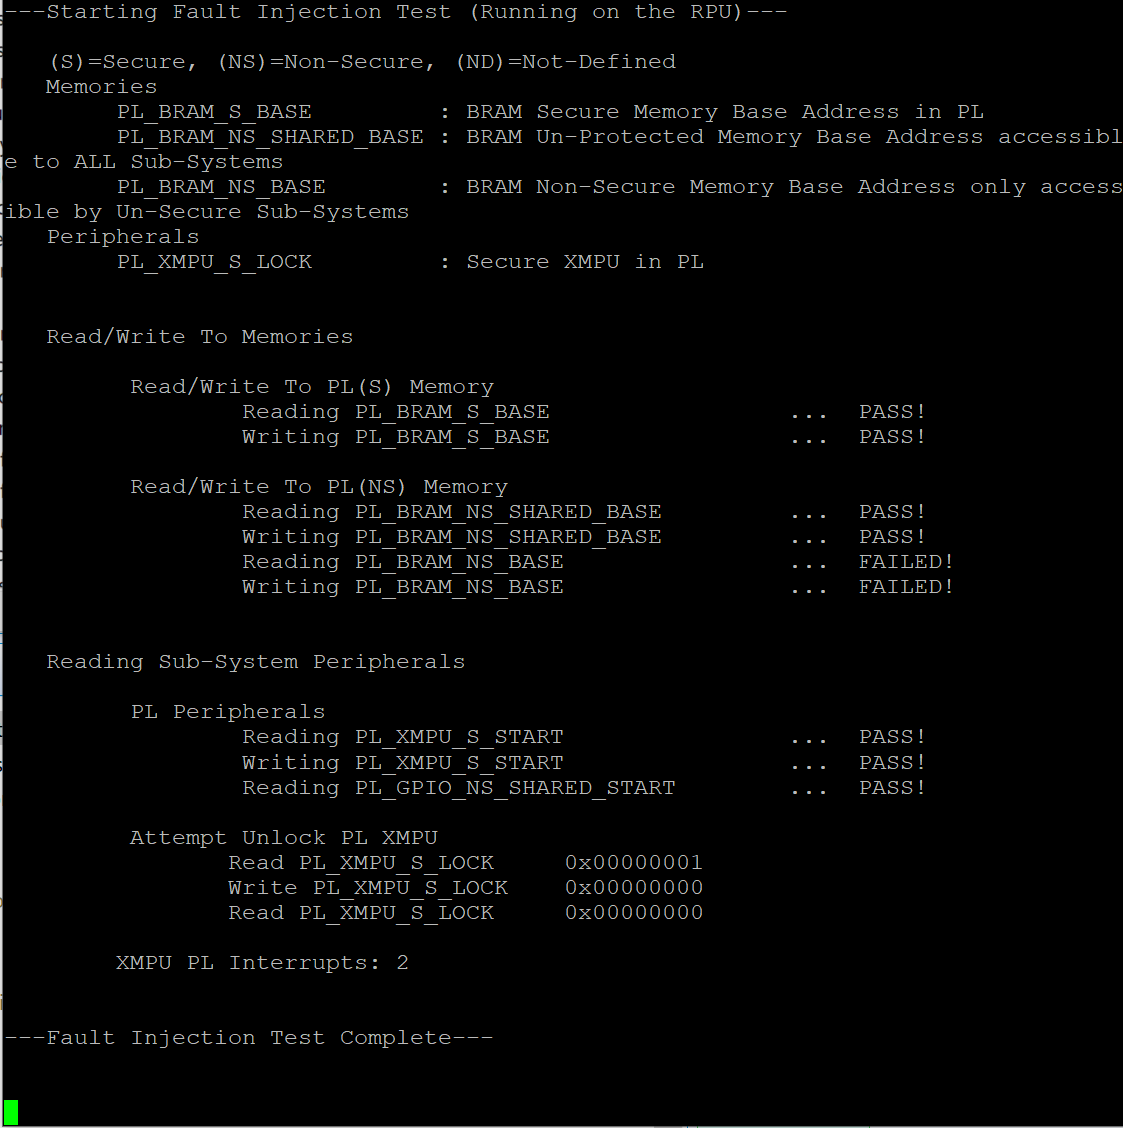
\includegraphics[width=\textwidth]{RPU_FI/RPU}
        \caption{RPU PL Read Attempt}
        \label{subfig:RPU_PLRead}
    \end{subfigure}
    \begin{subfigure}[b]{0.8\textwidth}
        \includegraphics[width=\textwidth]{RPU_FI/PMU.png}
        \caption{PMU Response to RPU PL Read Attempt}
        \label{subfig:RPU_PMU_Response}
    \end{subfigure}
    \caption{RPU Test Suite}
    \label{fig:RPU_Test_Suite}
\end{figure}

\section{Proposed Memory Isolation Design}\label{sec:DMADesign}

The memory isolation scheme proposed by this research effort is depicted in Figure \ref{fig:XMPU-PLDesign}. As can be seen in the figure, the PL is laid out in a star-like design, with the processor interface (through which the various partitions are administered) at its core. Data from the processor interface is directed through an interconnect IP, which acts as a crossbar switch to route data to the appropriate target. From this interconnect, data flows through one of a series of XMPU-PL units, one per tenant partition, before entering a second interconnect from which data is distributed within the partition. In this way, data is free to flow between devices within a partition (over this internal interconnect), but all requests from external resources are constrained to trusted system components by the XMPU-PL. The configuration registers of this XMPU-PL are configured such that either the supervisory processes (the scheduler, etc.) or the tenant themselves (presumably through a configuration interface on the processor) can modify them. That way, the tenant can grant access to system peripherals that are needed for its operation, such as Ethernet interfaces, or allow certain PS devices access if desired.

Meanwhile, the static components (the AES and KAC cores, as well as the partial reconfiguration (DFX) controller) are similarly connected to XMPU-PL cores, but said cores are not configured in the same way as those restricting tenant components. As they are part of the trusted static partition, there is not a need for constraining the memory space these cores can access. However, there is a a need to restrict what portions of the system can access them - specifically, only the EDF Scheduler and its associated interfaces, as outlined in Chapter \ref{ch:edfScheduling}, have a legitimate need for these cores. 

Accordingly, this functionality would, in the comprehensive design, be located in an isolated execution environment, which could be granted ``Secure'' status within the TrustZone framework. By then constraining the decryption cores and the DFX Controller as secure resources, it is possible to prevent malicious access to these resources. To this end, the configuration registers of these cores are locked, and only trusted components (such as the Scheduler), can access them. Such access could be necessary in order to allow the Scheduler and its associated interfaces to alter the memory regions with which the AES core may interface, such as when it is reallocated to a new core.

Finally, an additional XMPU-PL is located downstream of the tenant partition, enabling restriction of the tenant's AXI Masters to solely those memory regions and peripherals to which it is entitled access (those allocated specifically to its partition). Like the XMPU-PL cores protecting the static components, the configuration registers of this core are locked, and the tenant has no capability to override these locks in an attempt to allow additional access. 

\begin{figure}[H]
    \centering
    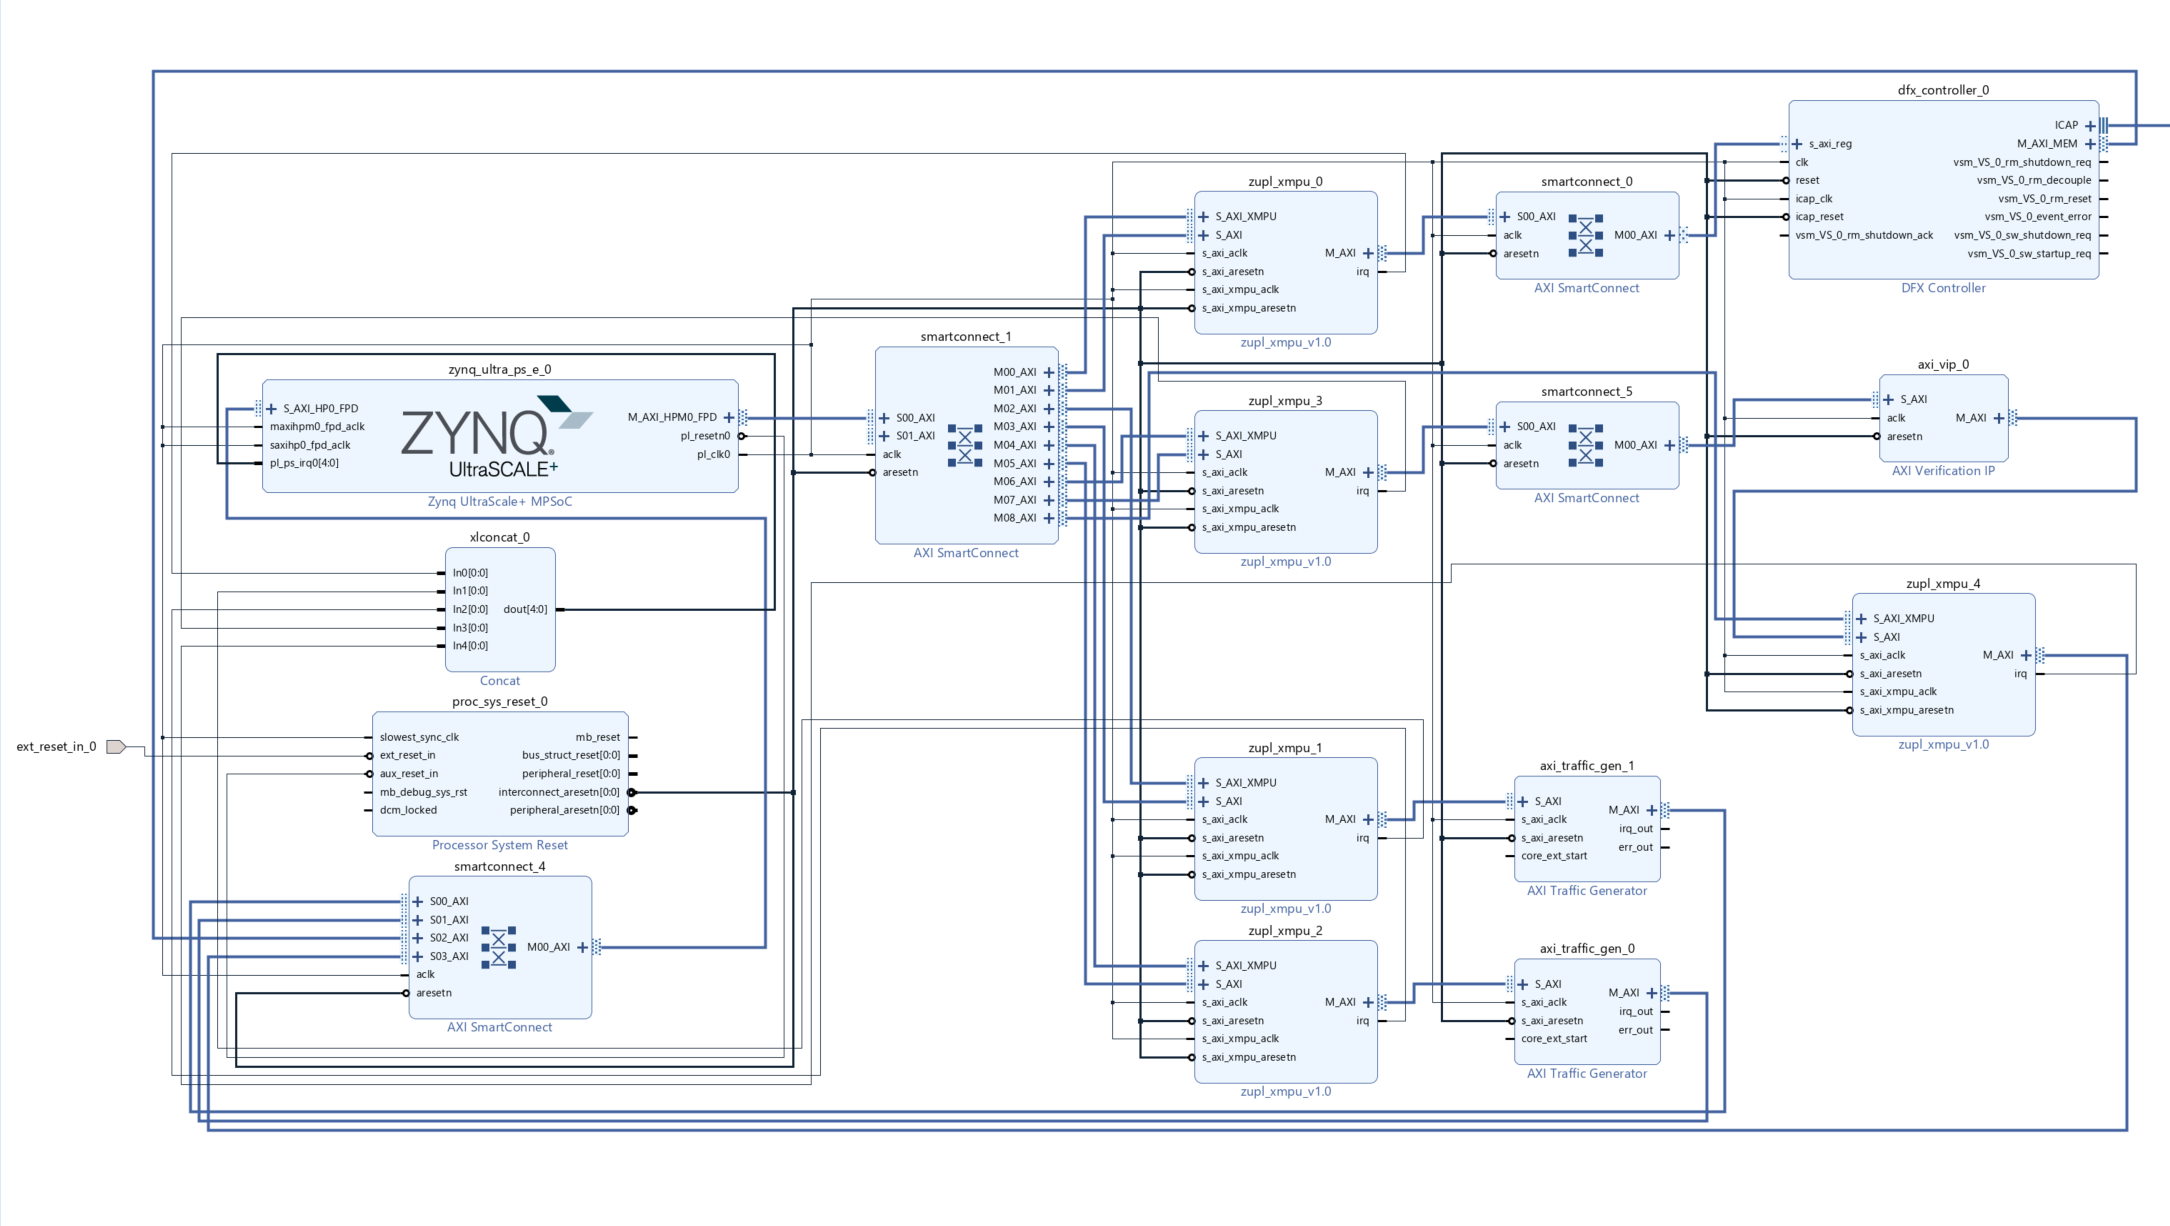
\includegraphics[width=.93\textheight, angle=90]{isolation_bd.png}
    \caption [Proposed XMPU-PL Design]{Xilinx Memory Protection Unit for Programmable Logic (XMPU-PL) in a Zynq UltraScale+ MPSoC architecture}
    \label{fig:XMPU-PLDesign}
\end{figure}

It should be acknowledged that the block diagram presented in Figure \ref{fig:XMPU-PLDesign} is necessarily simplified from what an actual CSP's implementation would afford. For starters, the design utilizes a pair of AXI Traffic Generator cores as stand-ins for a KAC engine and an AES engine, respectively. This is to enable a focus specifically on the memory isolation in this design, as opposed to attempting to implement a full architecture (and due to the lack of a licensed AES core, or any available KAC core in academia or industry). Additionally, it should be noted that this design only implements a single AES-representative core, and similarly only a single Dynamic Partial Reconfiguration Controller, where a more realistic implementation would include several AES engines (per the scheduler outlined in Chapter \ref{ch:edfScheduling}, above), as well as a separate Dynamic Partial Reconfiguration controller for each tenant partition. 

Similarly, the AXI Verification IP, located in the upper right portion of the diagram, is a stand-in for whatever user logic might be implemented in the tenant bitstream. This is the cause of the AXI Interconnect located adjacent to this IP, which seems extraneous given that it has only a single input and a single output. In reality, this IP would be located within the tenant partition, and would allow for various tenant devices to share the common entry point into the partition.

\subsection{Memory Regions in Proposed Design}\label{subsec:DMAMemRegions}
One of the key functions of the XMPU-PL is the ability to constrain upstream device access to specific regions of the overall memory map, thereby enabling isolation in excess of the traditional Secure/Non-secure binary dynamic. To take advantage of this functionality, the various XMPU-PL cores are configured with a variety of memory regions, which are divided at the system level in accordance with the table below. Note that these resources are at present constrained by the target hardware, which is discussed in detail in Section \ref{subsec:DMAEnvironmentHW}. These memory ranges are detailed in Table \ref{table:DMARanges}.

\begin{table}[ht!]
    \centering\begin{tabular}{|c|c|c|c|c|}
        \hline
        Region Purpose & Start Address & Width & Permitted Devices & Secure \\
        \hline
        PS Non-Secure Reserved & 0x00000000 & 1G & Sched/SM/Oth. PS & No \\
        PS Secure Reserved & 0x10000000 & 512M & Sched/SM/Oth. PS & Yes \\
        AES Key (Encrypted) & 0x90000000 & 64K & Sched/SM/KAC & Yes \\
        AES Key (Decrypted) & 0x90010000 & 64K & Sched/SM/KAC/AES & Yes \\
        Tenant Bitstream  (Encrypted) & 0x90020000 & 64M & Sched/SM/AES & Yes \\
        Tenant Bitstream  (Decrypted) & 0x94020000 & 64M & Sched/SM/AES/DFXC & Yes \\
        Tenant Storage & 0x98020000 & 128M & Tenant & No \\
        DFX Controller Config & 0xA0000000 & 64K & Sched/SM & Yes \\
        DFXC XMPU-PL Config & 0xA0010000 & 64K & Sched/SM & Yes \\
        AES XMPU-PL Config & 0xA0020000 & 64K  &Sched/SM & Yes \\
        KAC XMPU-PL Config & 0xA0030000 & 64K & Sched/SM & Yes \\
        KAC Engine Config & 0xA0040000 & 64K & Sched/SM & Yes \\
        AES Engine Config & 0xA0050000 & 64K & Sched/SM & Yes \\
        Tenant XMPU-PL Config (US) & 0xA0060000 & 64K & Sched/SM/Tenant & No \\
        Tenant XMPU-PL Config (DS) & 0xA0070000 & 64K & Sched/SM & No \\
        \hline
    \end{tabular}
    \caption{Memory Ranges in the Isolation Design}
    \label{table:DMARanges}
\end{table}

It should be noted that several of these ranges are appreciably larger than are needed, especially for configuration register spaces with a countably small number of registers. In these cases, these address ranges were assigned out of convenience of numerical value, as well as to allow for flexibility should future iterations of those components require additional register space. Such spaces could certainly be optimized should more space be required in a final design.

\section{Development and Test Environment}\label{sec:DMAEnvironment}

\subsection{Development Environment}\label{subsec:DMAEnvironmentDev}
The design presented in \ref{fig:XMPU-PLDesign} was implemented utilizing the same developer machine as outlined in \ref{subsec:devEnv}. Specifically, the development machine used by the authors in the course of this project was a Windows 10 Professional Edition 64-bit laptop featuring an Intel Core i7-9750H CPU with a base frequency of 2.60GHz. The machine featured 16 GB of DDR4 DRAM and a 1 TB SSD. Furthermore, the build process utilized the same Docker container as outlined in \ref{subsec:devEnv} to facilitate the development of the design.

\subsection{Target Hardware}\label{subsec:DMAEnvironmentHW}
Unlike the previous design, the desired use of the UltraScale+ architecture, with all of the isolation benefits outlined above, required the transition of the research effort away from the use of the ZedBoard as a hardware platform of choice. Instead, this effort targeted a recently released development platform that provides an affordable UltraScale+ MPSoC system, the Alinx AXU2CGB. The AXU2CGB, depicted in Figure \ref{fig:AXU2CGB}, is a compact development platform that includes an XCZU2CG-1SFVC784E UltraScale+ MPSoC. This MPSoC integrates a Dual-Core ARM Cortex-A53 Application Processor with a Dual-Core ARM Cortex-R5 Real Time Processor, combined with an FPGA that boasts over 103,000 logic cells, 94,000 look up tables, 240 DSP slices, 5.3 Mb of Block RAM, and 32MB of QSPI Flash. The larger AXU2CGB board also provides 2 GB of DDR4 RAM, as well as an 8GB EMMC Flash device.

\begin{figure}
    \centering
    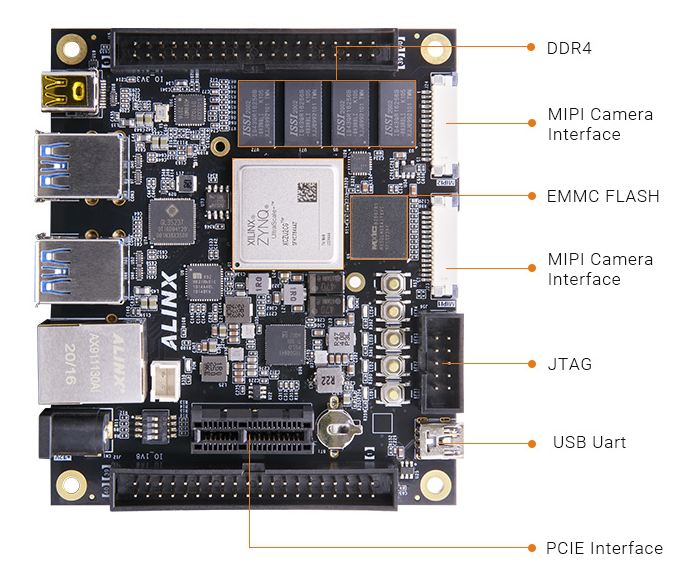
\includegraphics[]{axu2cgb.png}
    \caption[AXU2CGB Development System]{Alinx AXU2CGB Development System, with key components highlighted \cite{noauthor_axu2cgb_nodate}}
    \label{fig:AXU2CGB}
\end{figure}

\subsection{Target Operating System}\label{subsec:DMAEnvironmentOS}
Although the integration of the architecture depicted in Figure \ref{fig:XMPU-PLDesign} into a larger system integrating the PS-based scheduler outlined in Chapter \ref{ch:edfScheduling} would necessitate a PetaLinux (or similar) environment, the isolated development of this functionality as outlined in this section does not strictly necessitate a full-featured operating system be implemented for its verification. Furthermore, the XMPU-PL was not presented by Xilinx with accompanying Linux-compatible drivers, which necessarily differ from those used in a ``Standalone'' configuration. To this end, this effort chose to implement and exercise this design in such a standalone environment. 

Care should be taken in applying the phrase ``Standalone'' to this design. In a traditional sense, this would indicate that the target application (in this case, test software to exercise the XMPU-PL) is compiled directly to ARM instructions, which execute immediately following the application of power to the system. However, the MPSoC is sufficiently complex that such an assumption would be unwieldy. To this end, what Xilinx calls a ``Standalone'' project is actually a project that utilizes its Standalone library, which it describes as ``a single-threaded, simple operating system (OS) platform that provides the lowest layer of software modules used to access processor-specific functions'' \cite{noauthor_os_2020}.
% Much like the ZedBoard, the AXU2CGB is well suited for the PetaLinux operating environment provided by Xilinx for use on its SoCs. Initial efforts targeting this board have utilized the stock PetaLinux image provided with the purchase of the board, which is based on the same PetaLinux 2020.2 toolchain as previously discussed. Later efforts implementing various test applications have utilized slightly modified variants, which are discussed in subsequent sections. Additionally, certain tests were conducted in a ``bare-metal'' environment, wherein the applications were executed directly on the target without an operating system serving as a middle layer.

\section{Implementation Results}\label{sec:DMAResults}

The direct experimental results of the implementation of the architecture outlined in Figure \ref{fig:XMPU-PLDesign}, above, consist of serial interface printouts that very nearly mirror Figures \ref{fig:APU_Test_Suite} and \ref{fig:RPU_Test_Suite}, above. Accordingly, they are not included herein for purposes of brevity. However, one immediate takeaway from the implementation of the design shown in Figure \ref{fig:XMPU-PLDesign}, above, is that it consumes a large portion of the available PL, even on a recent (and comparatively large) FPGA such as the one afforded by the AXU2CGB. As the utilization report shown in Figure \ref{fig:XMPU-PLUtilization} shows, nearly 95\% of all Look Up Tables (LUTs) are consumed in this design. However, it should be noted that such an FPGA is appreciably smaller still than the large format devices that will likely become the tool of choice for cloud based operations, and in such instances this design yields appreciable savings over the previously proposed architectures. Furthermore, a portion of this utilization is consumed by the AXI Traffic Generator IPs acting as stand-ins for the KAC and AES engines, as well as for the verification IP standing in for the user logic. The resources consumed by these cores should not be taken as representative of the actual IP they are intended to act as a substitute for.

\begin{figure}
    \centering
    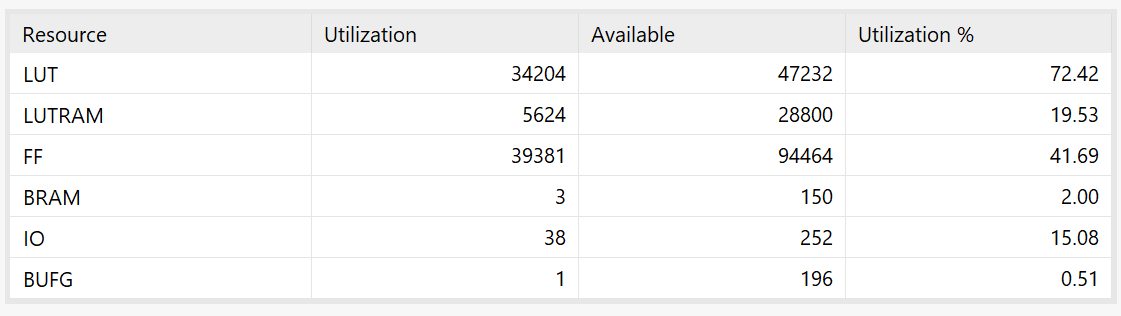
\includegraphics[width=0.5\textwidth]{xmpupl_utilization.png}
    \caption[Memory Isolation Resource Utilization]{Resource Utilization for the XMPU-PL design, as implemented on the AXU2CGB}
    \label{fig:XMPU-PLUtilization}
\end{figure}

Furthermore, it should be noted that the current implementation of the design still utilizes the isolation architecture implemented in the reference designs, wherein the PMU acts in the supervisory capacity, detecting rejected transactions from the PL. In the context of the larger reference design, it is likely that this functionality would be located within one of the hard processing systems, likely within the APU as the security monitor functionality would likely require multithreading, a function not afforded by the MMU-less Cortex-R5 cores. As was discussed earlier in this chapter, such a migration would require the implementation of custom Linux drivers for the IP, as it is currently provided with drivers only for the standalone environment.